\chapter{Hasil Pengujian Eksperimental}
\label{chap:hasilpengujianeksperimental}

Hasil pengujian eksperimental ini berupa bagan yang dibuat dari data pada Lampiran \ref{chap:datahasilpengujian}. Berikut adalah bagan hasil dari pengujian eksperimental :

\begin{figure}[H]
				\centering		
				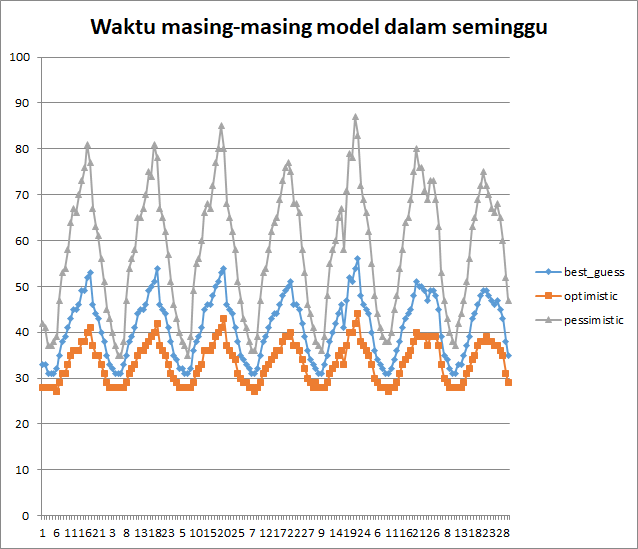
\includegraphics[scale=0.7]{Gambar/waktuallmodelsampel117072017normal.png}
\end{figure}
\newpage
			
\begin{figure}[H]
				\centering		
				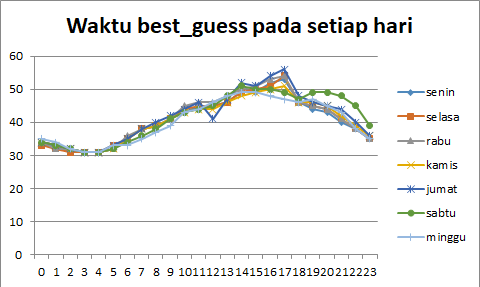
\includegraphics[]{Gambar/waktubestguesssampel117072017normal.png}
				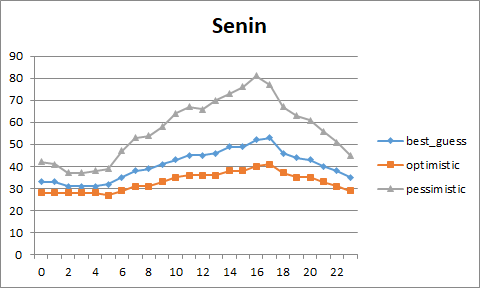
\includegraphics[]{Gambar/seninsampel117072017normal.png}
				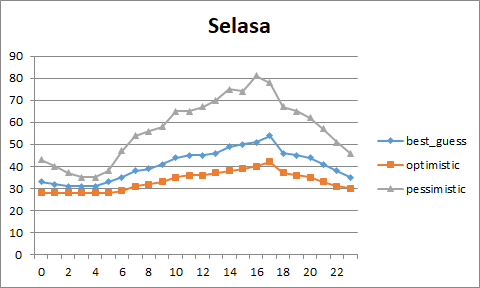
\includegraphics[]{Gambar/selasasampel117072017normal.png}
\end{figure}			
			
\begin{figure}[H]
				\centering		
				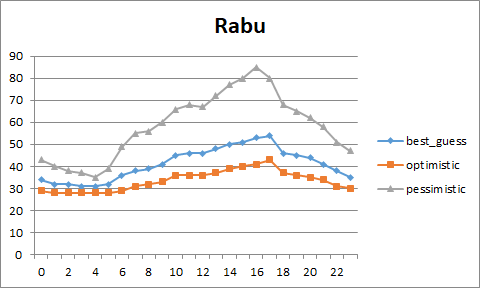
\includegraphics[]{Gambar/rabusampel117072017normal.png}
				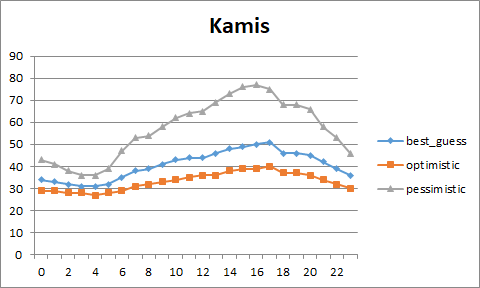
\includegraphics[]{Gambar/kamissampel117072017normal.png}
				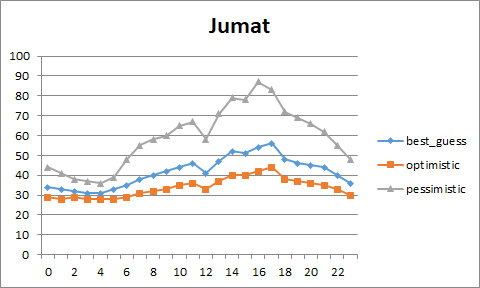
\includegraphics[]{Gambar/jumatsampel117072017normal.png}
\end{figure}	
			
\begin{figure}[H]
				\centering	
				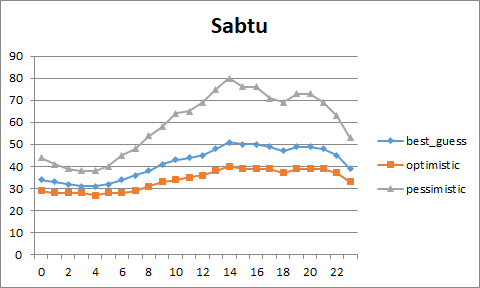
\includegraphics[]{Gambar/sabtusampel117072017normal.png}
				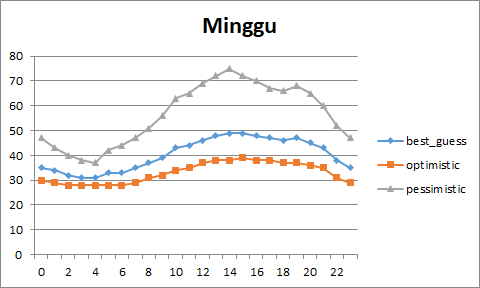
\includegraphics[]{Gambar/minggusampel117072017normal.png}
				\caption[Hasil Pengujian Eksperimental]{Hasil Pengujian Eksperimental sampel 1 17 Juli Mei 2017 dengan alamat yang tidak ditukar}
				\label{fig:eksperimentalsampel117072017normal}
\end{figure}

\newpage
				
\begin{figure}[H]
				\centering		
				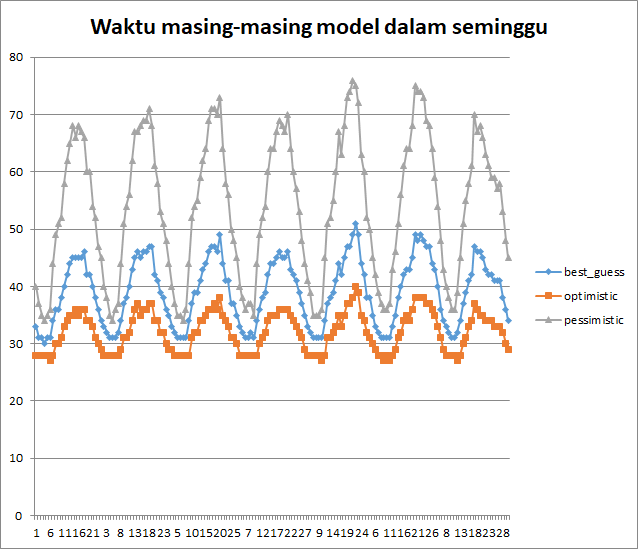
\includegraphics[scale=0.7]{Gambar/waktuallmodelsampel117072017reverse.png}
				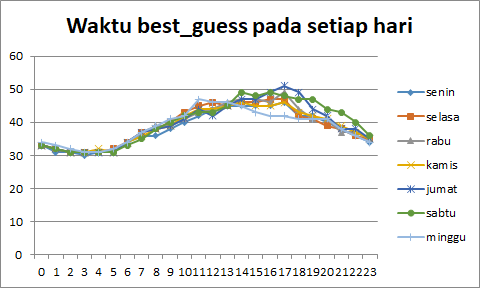
\includegraphics[]{Gambar/waktubestguesssampel117072017reverse.png}
				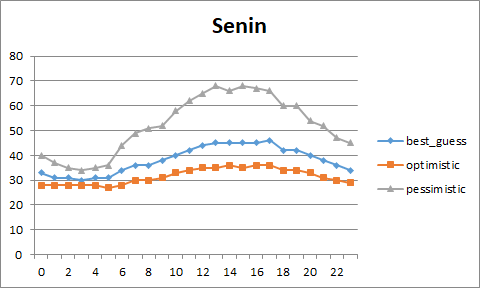
\includegraphics[]{Gambar/seninsampel117072017reverse.png}
\end{figure}
			
\begin{figure}[H]
				\centering		
				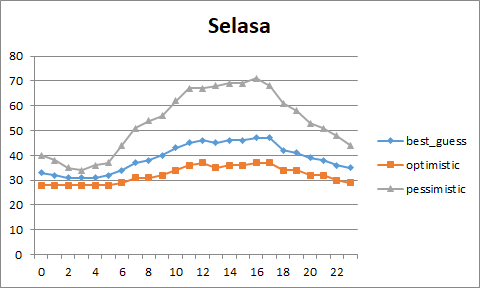
\includegraphics[]{Gambar/selasasampel117072017reverse.png}
				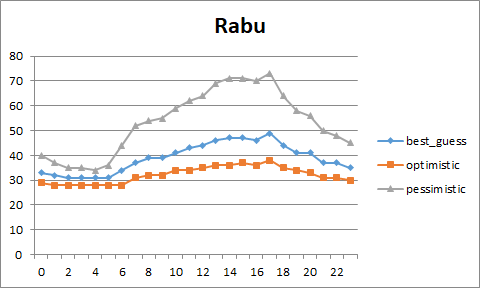
\includegraphics[]{Gambar/rabusampel117072017reverse.png}
				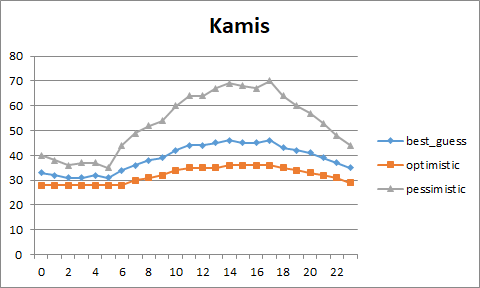
\includegraphics[]{Gambar/kamissampel117072017reverse.png}
\end{figure}			
			
\begin{figure}[H]
				\centering		
				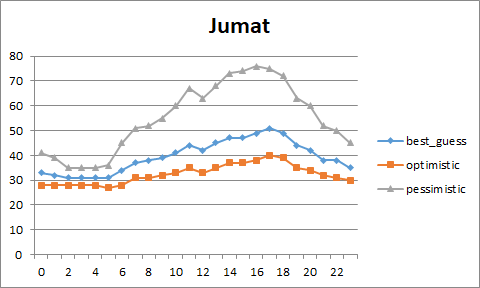
\includegraphics[]{Gambar/jumatsampel117072017reverse.png}
				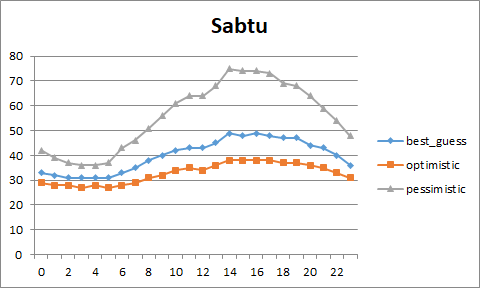
\includegraphics[]{Gambar/sabtusampel117072017reverse.png}
				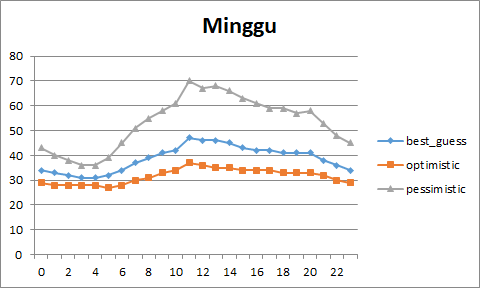
\includegraphics[]{Gambar/minggusampel117072017reverse.png}
				\caption[Hasil Pengujian Eksperimental]{Hasil Pengujian Eksperimental sampel 1 17 Juli 2017 dengan alamat yang ditukar}
				\label{fig:eksperimentalsampel117072017reverse}
\end{figure}	
\newpage
			
\begin{figure}[H]
				\centering		
				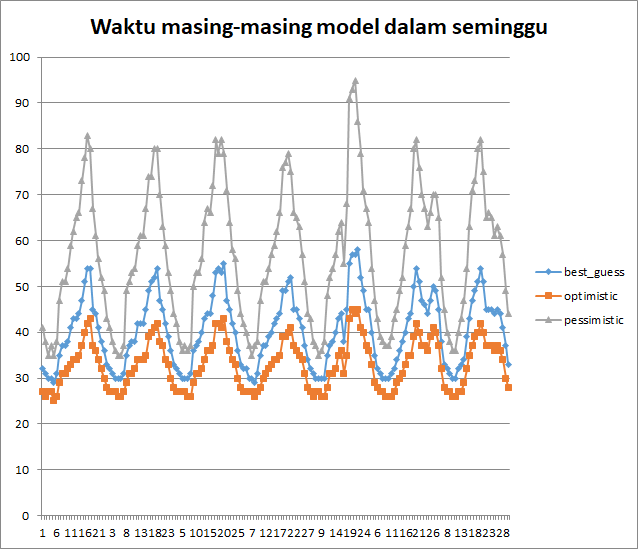
\includegraphics[scale=0.7]{Gambar/waktuallmodelsampel217072017normal.png}
				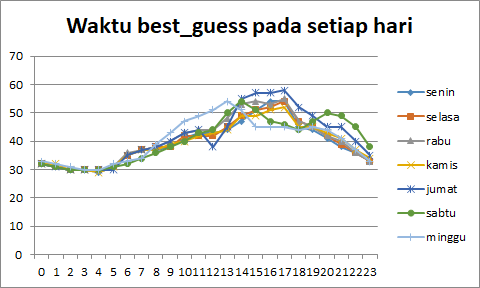
\includegraphics[]{Gambar/waktubestguesssampel217072017normal.png}
				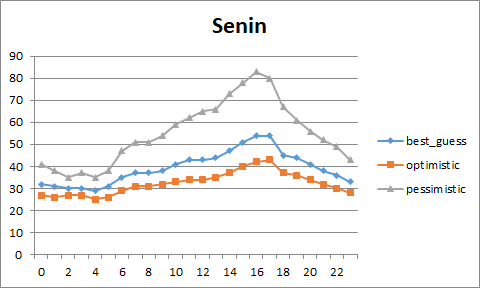
\includegraphics[]{Gambar/seninsampel217072017normal.png}
\end{figure}
			
\begin{figure}[H]
				\centering		
				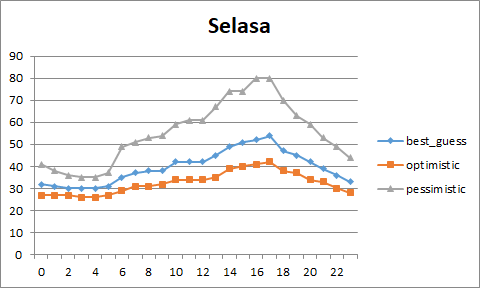
\includegraphics[]{Gambar/selasasampel217072017normal.png}
				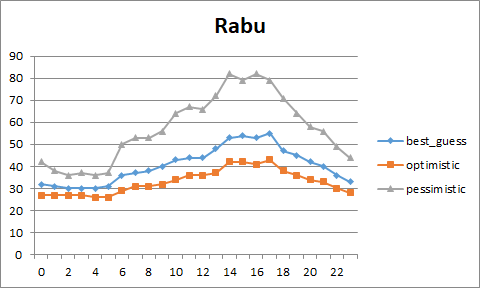
\includegraphics[]{Gambar/rabusampel217072017normal.png}
				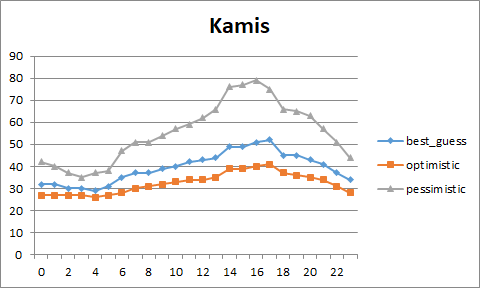
\includegraphics[]{Gambar/kamissampel217072017normal.png}
\end{figure}			
			
\begin{figure}[H]
				\centering		
				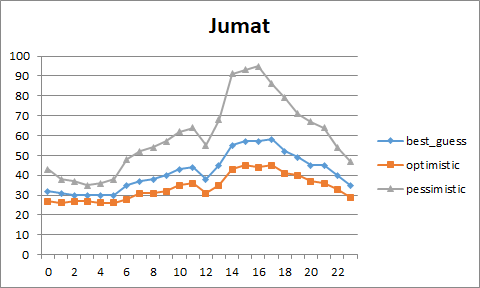
\includegraphics[]{Gambar/jumatsampel217072017normal.png}
				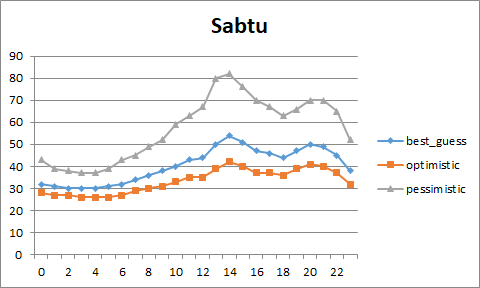
\includegraphics[]{Gambar/sabtusampel217072017normal.png}
				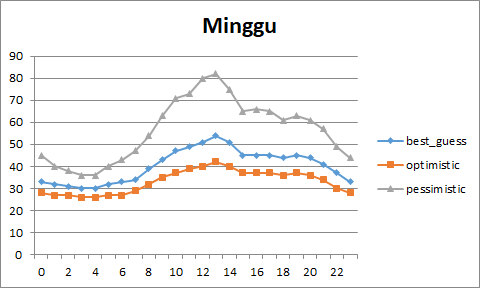
\includegraphics[]{Gambar/minggusampel217072017normal.png}
				\caption[Hasil Pengujian Eksperimental]{Hasil Pengujian Eksperimental sampel 2 17 Juli 2017 dengan alamat yang tidak ditukar}
				\label{fig:eksperimentalsampel217072017normal}
\end{figure}
\newpage
			
\begin{figure}[H]
				\centering		
				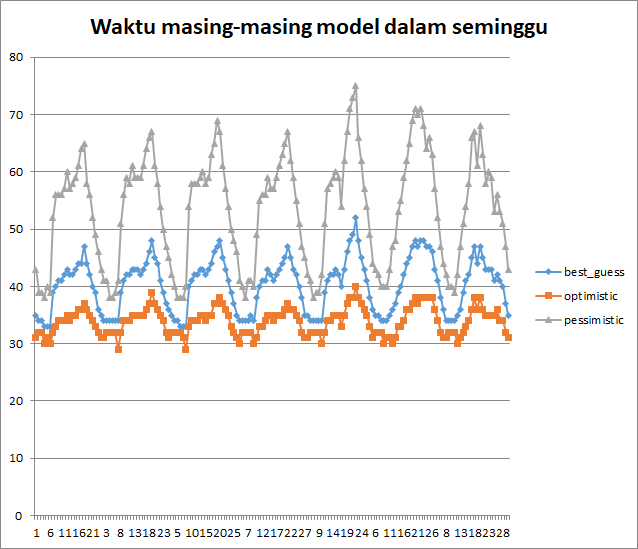
\includegraphics[scale=0.7]{Gambar/waktuallmodelsampel217072017reverse.png}
				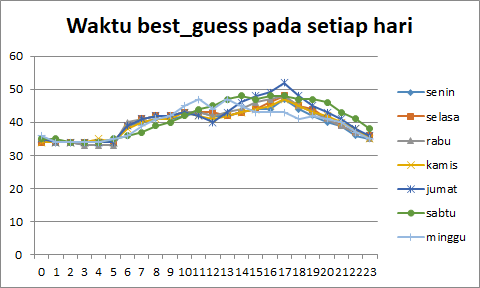
\includegraphics[]{Gambar/waktubestguesssampel217072017reverse.png}
				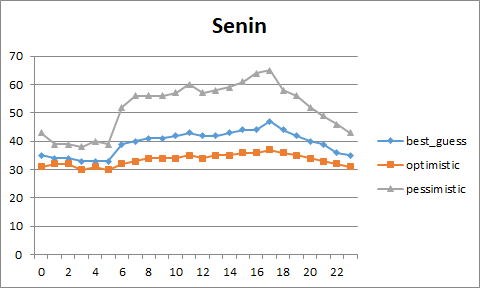
\includegraphics[]{Gambar/seninsampel217072017reverse.png}
\end{figure}
			
\begin{figure}[H]
				\centering		
				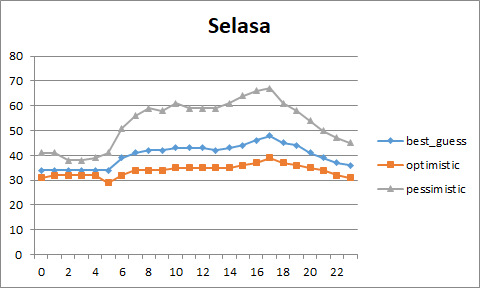
\includegraphics[]{Gambar/selasasampel217072017reverse.png}
				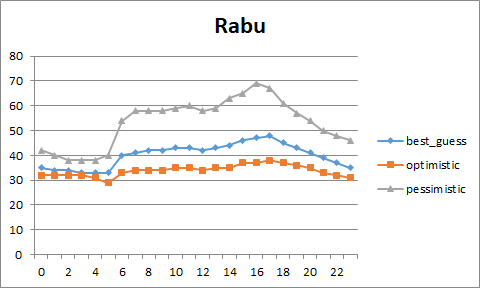
\includegraphics[]{Gambar/rabusampel217072017reverse.png}
				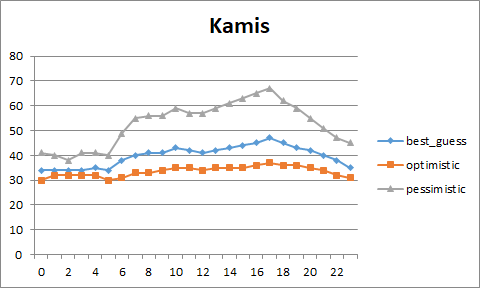
\includegraphics[]{Gambar/kamissampel217072017reverse.png}
\end{figure}			
			
\begin{figure}[H]
				\centering		
				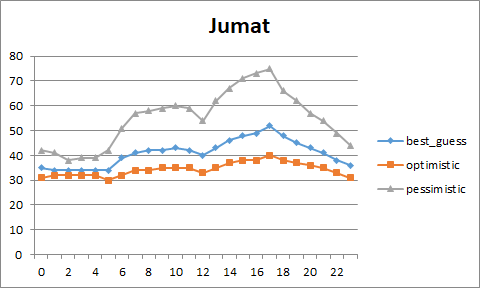
\includegraphics[]{Gambar/jumatsampel217072017reverse.png}
				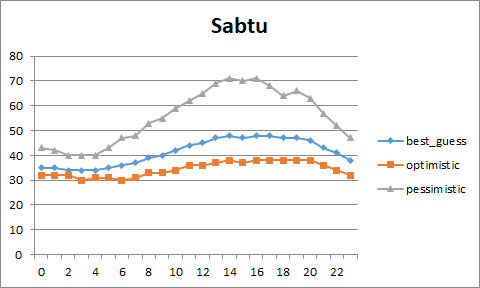
\includegraphics[]{Gambar/sabtusampel217072017reverse.png}
				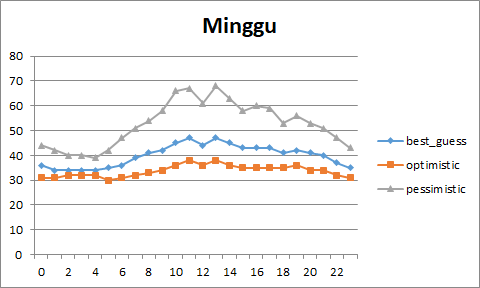
\includegraphics[]{Gambar/minggusampel217072017reverse.png}
				\caption[Hasil Pengujian Eksperimental]{Hasil Pengujian Eksperimental sampel 2 17 Juli 2017 dengan alamat yang ditukar}
				\label{fig:eksperimentalsampel217072017reverse}
\end{figure}

\begin{figure}[H]
				\centering		
				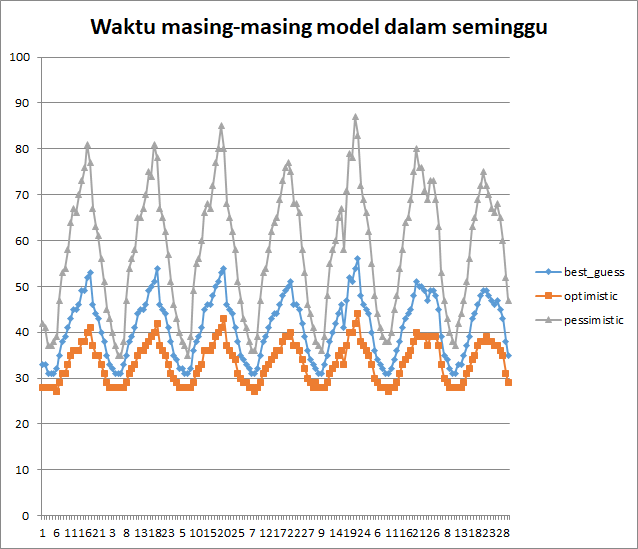
\includegraphics[scale=0.7]{Gambar/waktuallmodelsampel124072017normal.png}
				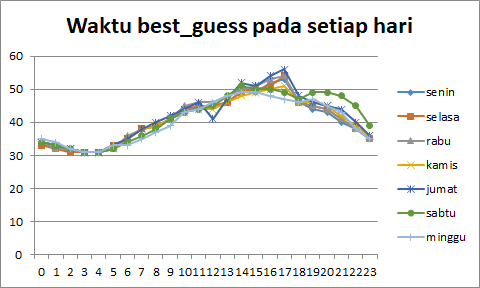
\includegraphics[]{Gambar/waktubestguesssampel124072017normal.png}
				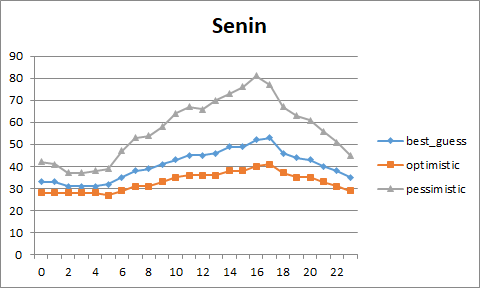
\includegraphics[]{Gambar/seninsampel124072017normal.png}
\end{figure}
			
\begin{figure}[H]
				\centering		
				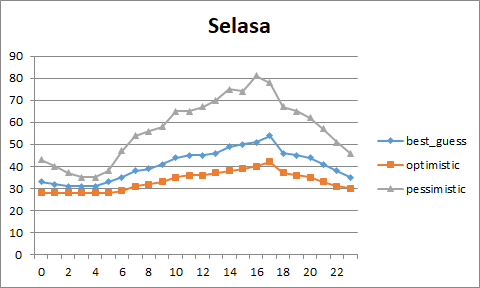
\includegraphics[]{Gambar/selasasampel124072017normal.png}
				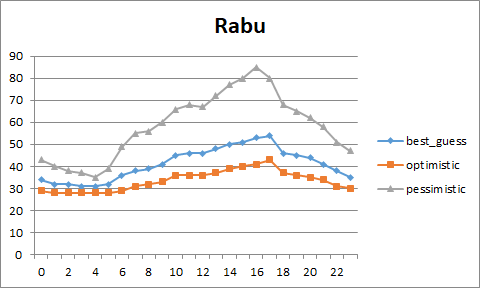
\includegraphics[]{Gambar/rabusampel124072017normal.png}
				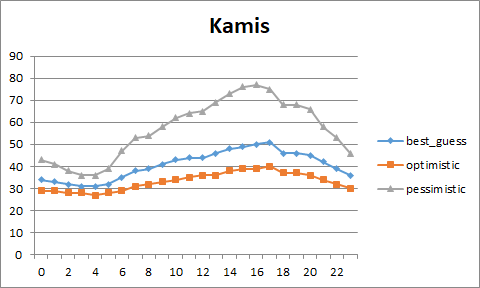
\includegraphics[]{Gambar/kamissampel124072017normal.png}
\end{figure}			
			
\begin{figure}[H]
				\centering		
				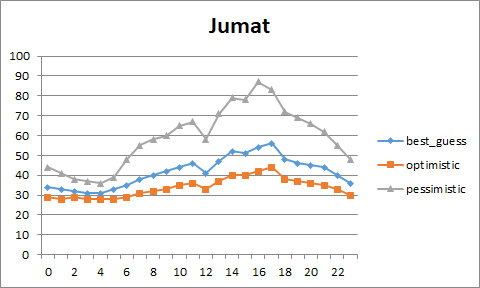
\includegraphics[]{Gambar/jumatsampel124072017normal.png}
				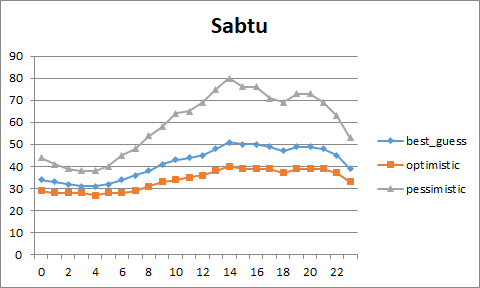
\includegraphics[]{Gambar/sabtusampel124072017normal.png}
				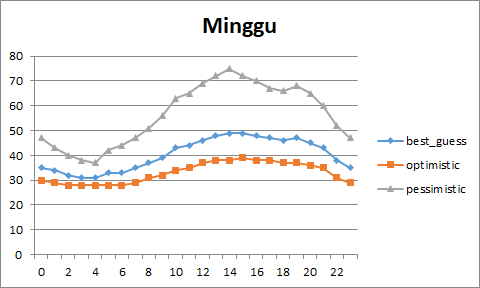
\includegraphics[]{Gambar/minggusampel124072017normal.png}
				\caption[Hasil Pengujian Eksperimental]{Hasil Pengujian Eksperimental sampel 1 24 Juli 2017 dengan alamat yang tidak ditukar}
				\label{fig:eksperimentalsampel2124072017normal}
\end{figure}

\begin{figure}[H]
				\centering		
				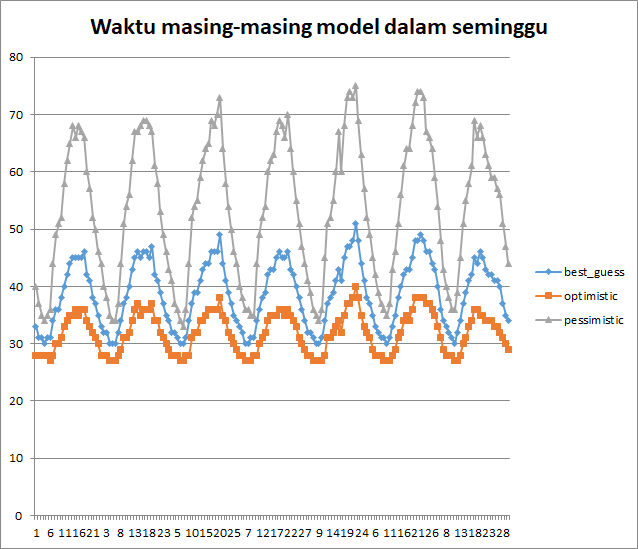
\includegraphics[scale=0.7]{Gambar/waktuallmodelsampel124072017reverse.png}
				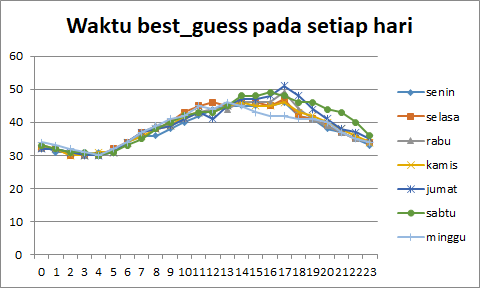
\includegraphics[]{Gambar/waktubestguesssampel124072017reverse.png}
				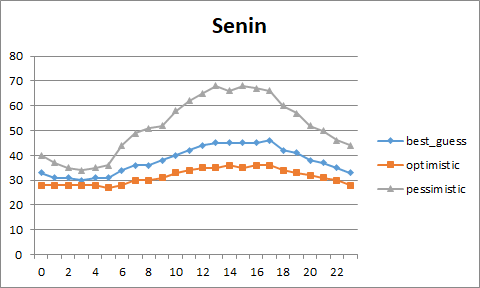
\includegraphics[]{Gambar/seninsampel124072017reverse.png}
\end{figure}
			
\begin{figure}[H]
				\centering		
				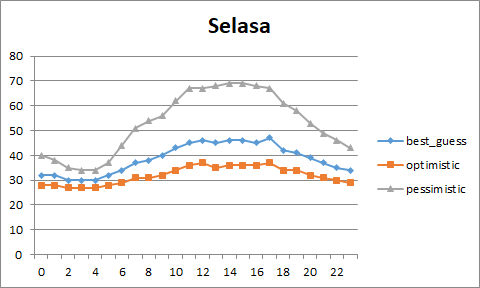
\includegraphics[]{Gambar/selasasampel124072017reverse.png}
				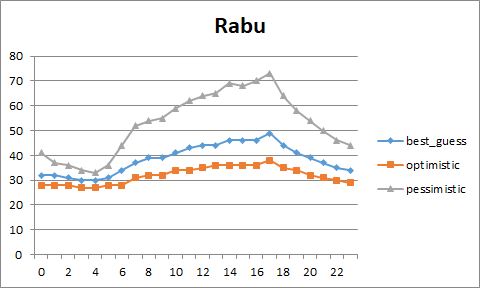
\includegraphics[]{Gambar/rabusampel124072017reverse.png}
				\includegraphics[]{Gambar/kamissampel124072017reverse.png}
\end{figure}			
			
\begin{figure}[H]
				\centering		
				\includegraphics[]{Gambar/jumatsampel124072017reverse.png}
				\includegraphics[]{Gambar/sabtusampel124072017reverse.png}
				\includegraphics[]{Gambar/minggusampel124072017reverse.png}
				\caption[Hasil Pengujian Eksperimental]{Hasil Pengujian Eksperimental sampel 1 24 Juli 2017 dengan alamat yang ditukar}
				\label{fig:eksperimentalsampel124072017reverse}
\end{figure}

\begin{figure}[H]
				\centering		
				\includegraphics[scale=0.7]{Gambar/waktuallmodelsampel224072017normal.png}
				\includegraphics[]{Gambar/waktubestguesssampel224072017normal.png}
				\includegraphics[]{Gambar/seninsampel224072017normal.png}
\end{figure}
			
\begin{figure}[H]
				\centering		
				\includegraphics[]{Gambar/selasasampel224072017normal.png}
				\includegraphics[]{Gambar/rabusampel224072017normal.png}
				\includegraphics[]{Gambar/kamissampel224072017normal.png}
\end{figure}			
			
\begin{figure}[H]
				\centering		
				\includegraphics[]{Gambar/jumatsampel224072017normal.png}
				\includegraphics[]{Gambar/sabtusampel224072017normal.png}
				\includegraphics[]{Gambar/minggusampel224072017normal.png}
				\caption[Hasil Pengujian Eksperimental]{Hasil Pengujian Eksperimental sampel 2 24 Juli 2017 dengan alamat yang tidak ditukar}
				\label{fig:eksperimentalsampel224072017normal}
\end{figure}

\begin{figure}[H]
				\centering		
				\includegraphics[scale=0.7]{Gambar/waktuallmodelsampel224072017reverse.png}
				\includegraphics[]{Gambar/waktubestguesssampel224072017reverse.png}
				\includegraphics[]{Gambar/seninsampel224072017reverse.png}
\end{figure}
			
\begin{figure}[H]
				\centering		
				\includegraphics[]{Gambar/selasasampel224072017reverse.png}
				\includegraphics[]{Gambar/rabusampel224072017reverse.png}
				\includegraphics[]{Gambar/kamissampel224072017reverse.png}
\end{figure}			
			
\begin{figure}[H]
				\centering		
				\includegraphics[]{Gambar/jumatsampel224072017reverse.png}
				\includegraphics[]{Gambar/sabtusampel224072017reverse.png}
				\includegraphics[]{Gambar/minggusampel224072017reverse.png}
				\caption[Hasil Pengujian Eksperimental]{Hasil Pengujian Eksperimental sampel 2 24 Juli 2017 dengan alamat yang ditukar}
				\label{fig:eksperimentalsampel224072017reverse}
\end{figure}